\documentclass[10pt,a4paper]{article}
\usepackage[utf8]{inputenc}
\usepackage{amsmath}
\usepackage{amsfonts}
\usepackage{amssymb}
\usepackage[left=2cm,right=2cm,top=2cm,bottom=2cm]{geometry}
\usepackage{graphicx}
\usepackage{wrapfig}
\usepackage{float}
\usepackage{braket}
\usepackage{mathtools}
\author{\begin{tabular}{rl}
\textbf{Course:} & PHYS 127AL \\
\textbf{Student Name:} & Nicholas Morrow \\
\textbf{Perm:} & 846646-8 \\
\end{tabular}}
\title{Progress Report - MIDI/CV Converter}

\begin{document}
	\begin{titlepage}
		\maketitle
		\tableofcontents
	\end{titlepage}

	\section{Background}
		The MIDI to CV converter provides a hardware-independent digital interface to the voltage-controlled elements of the synthesizer, allowing the unit to be controlled using standard MIDI-compliant controller equipment and eliminating the need for the development of a customized pitch-control interface.
	\section{Hardware}
		\subsection{Overview}
		\subsection{Input Stage}
				The input stage was taken directly from the MIDI 1.0 Specification, to ensure hardware compliance with industry equipment.
		\subsection{Signal Processing Stage}
			\subsubsection{MCU}
		\subsection{Output Stage}
			\subsubsection{DAC}
				The digital signal from the SPI output of the MCU is converted into an analog voltage by the MCP4921 DAC, from Microchip. The MCP4921 has 12-bit resolution, allowing for voltage adjustments in increments of $\frac{5}{2^{12}} \approx1.2$mV, which corresponds to a pitch resolution of $~3.22$ cents on the $1V/$oct control scale. The output resolution provided by the MCP4921 is sufficient for this application. 
				\begin{figure}[H]
					%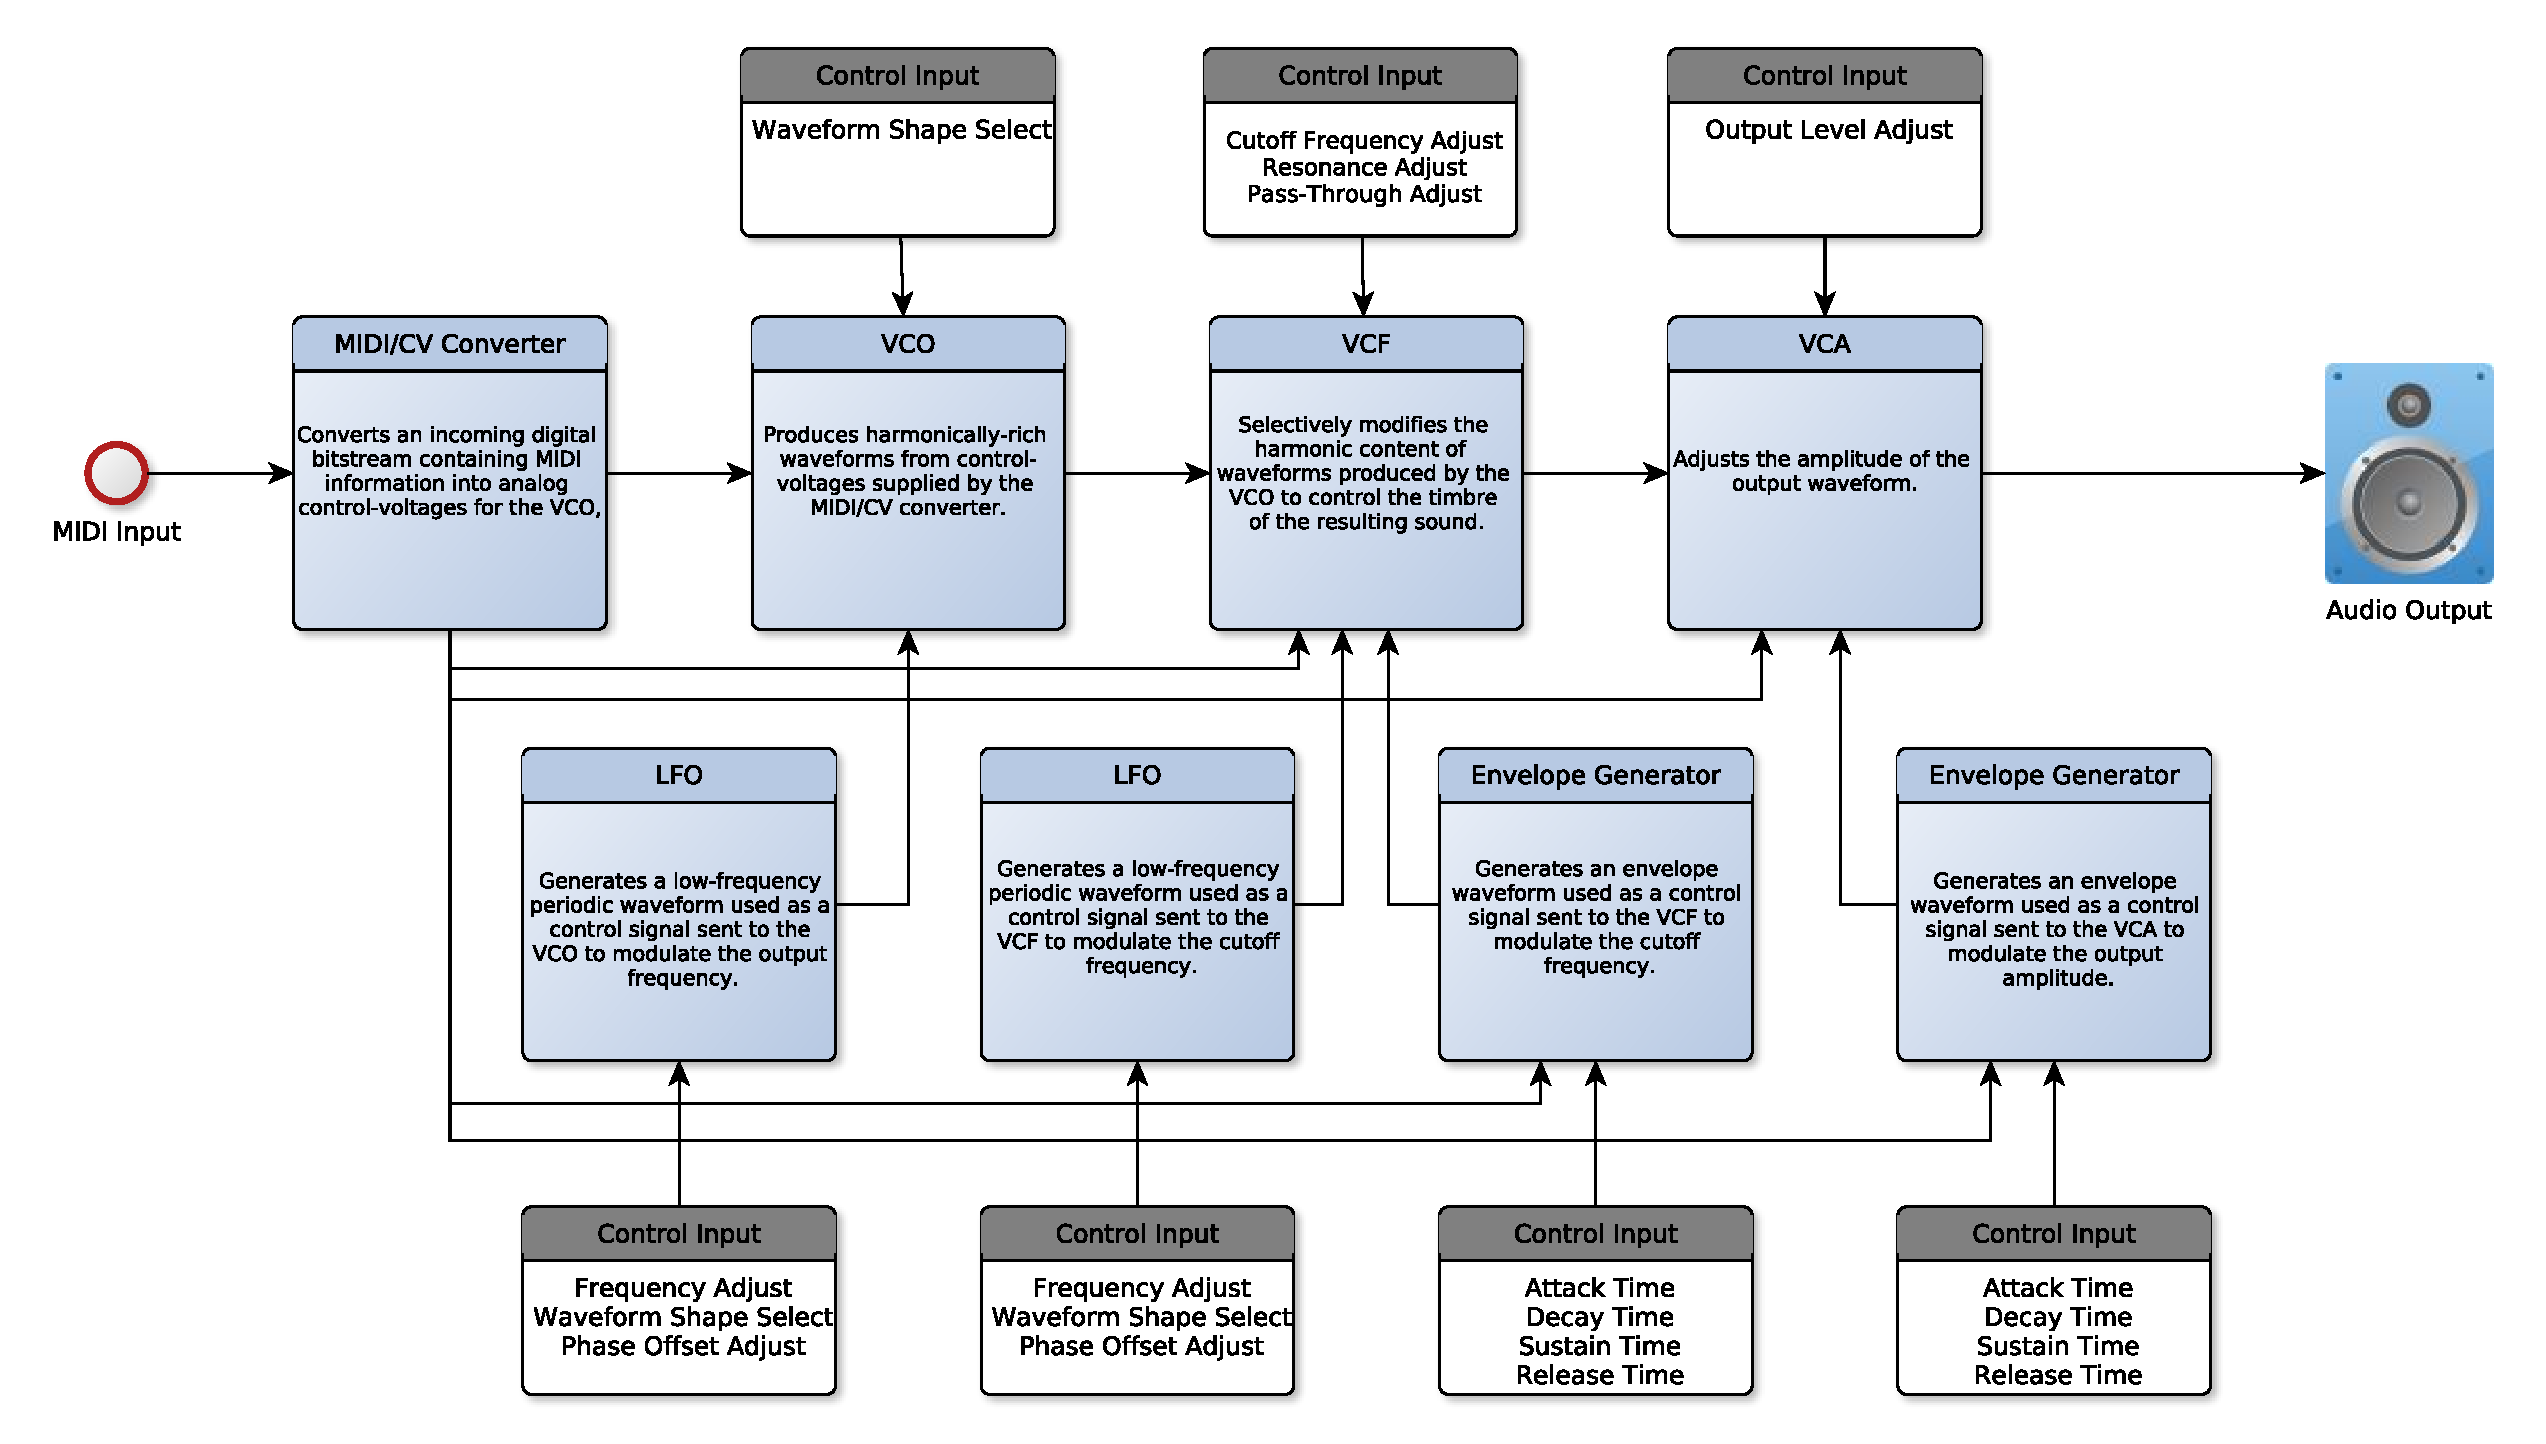
\includegraphics[width=\textwidth]{./figures/synthesizer.eps}
					\caption{MCP4921 DAC}
					\label{fig:dac}
				\end{figure}
			\subsubsection{Current Buffer}
				\begin{figure}[H]
					%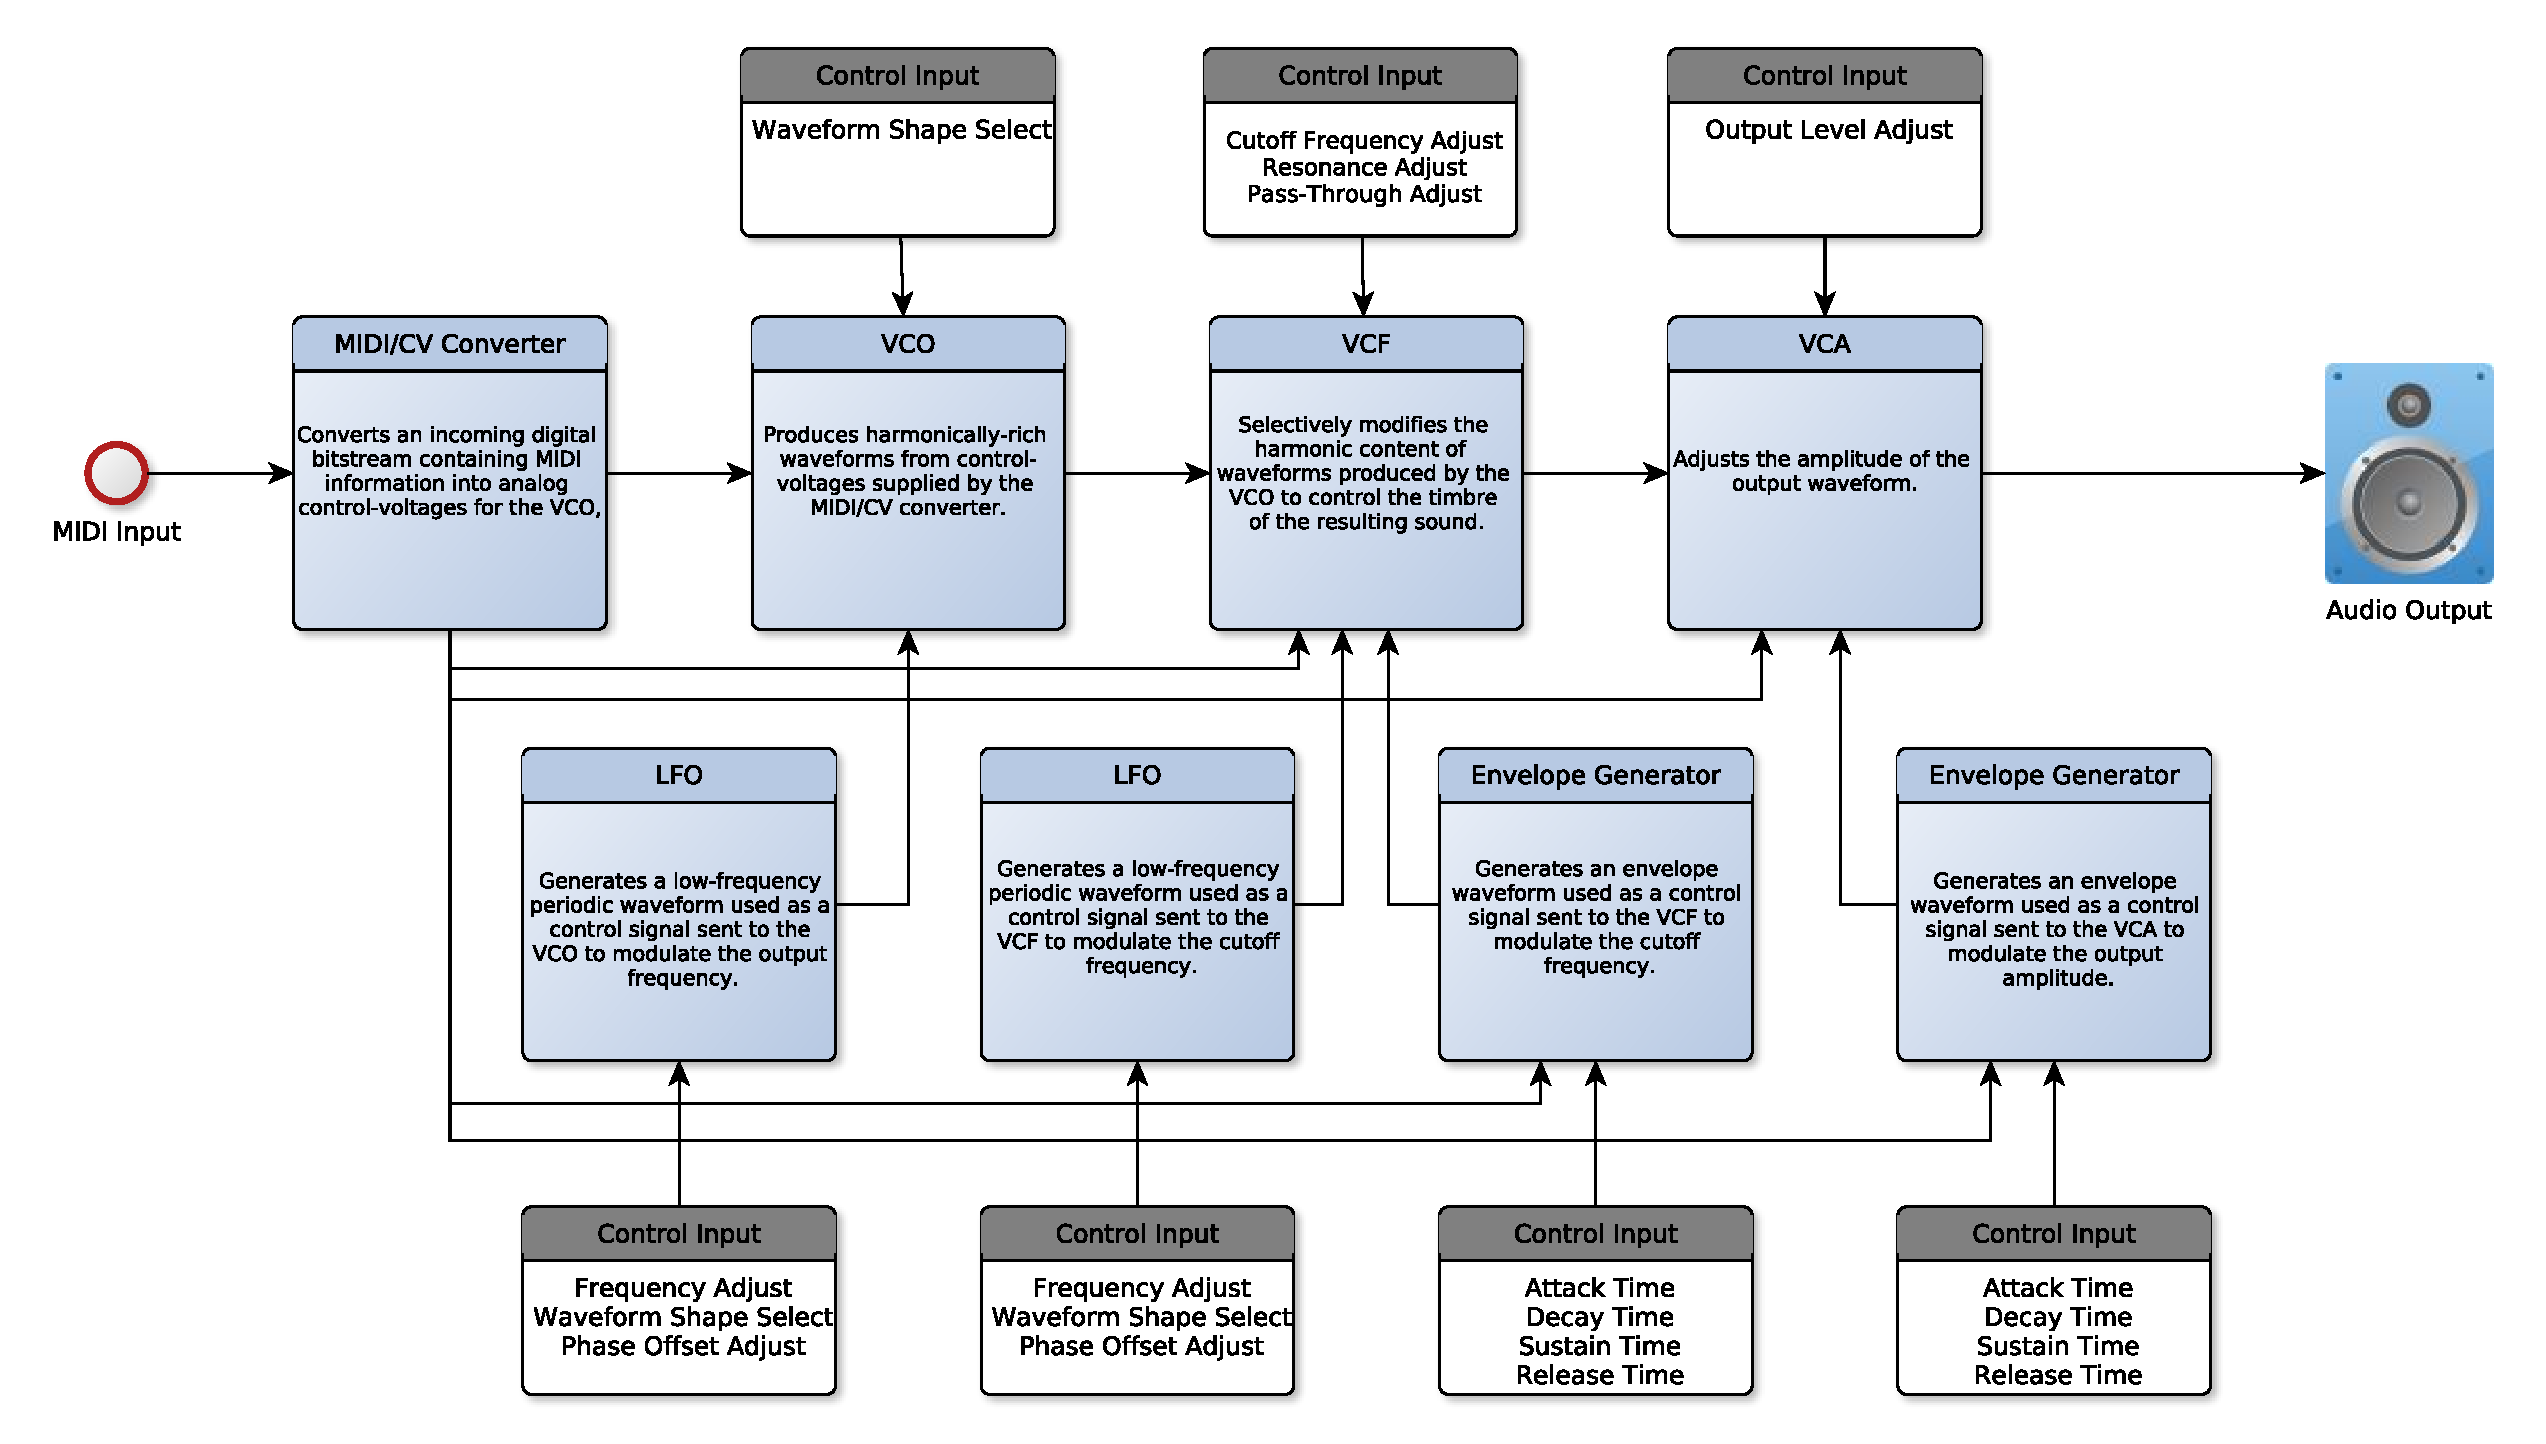
\includegraphics[width=\textwidth]{./figures/synthesizer.eps}
					\caption{Current Buffer}
					\label{fig:current_buffer}
				\end{figure}
			\subsubsection{Selectable Pitch Glide}
				\begin{figure}[H]
					%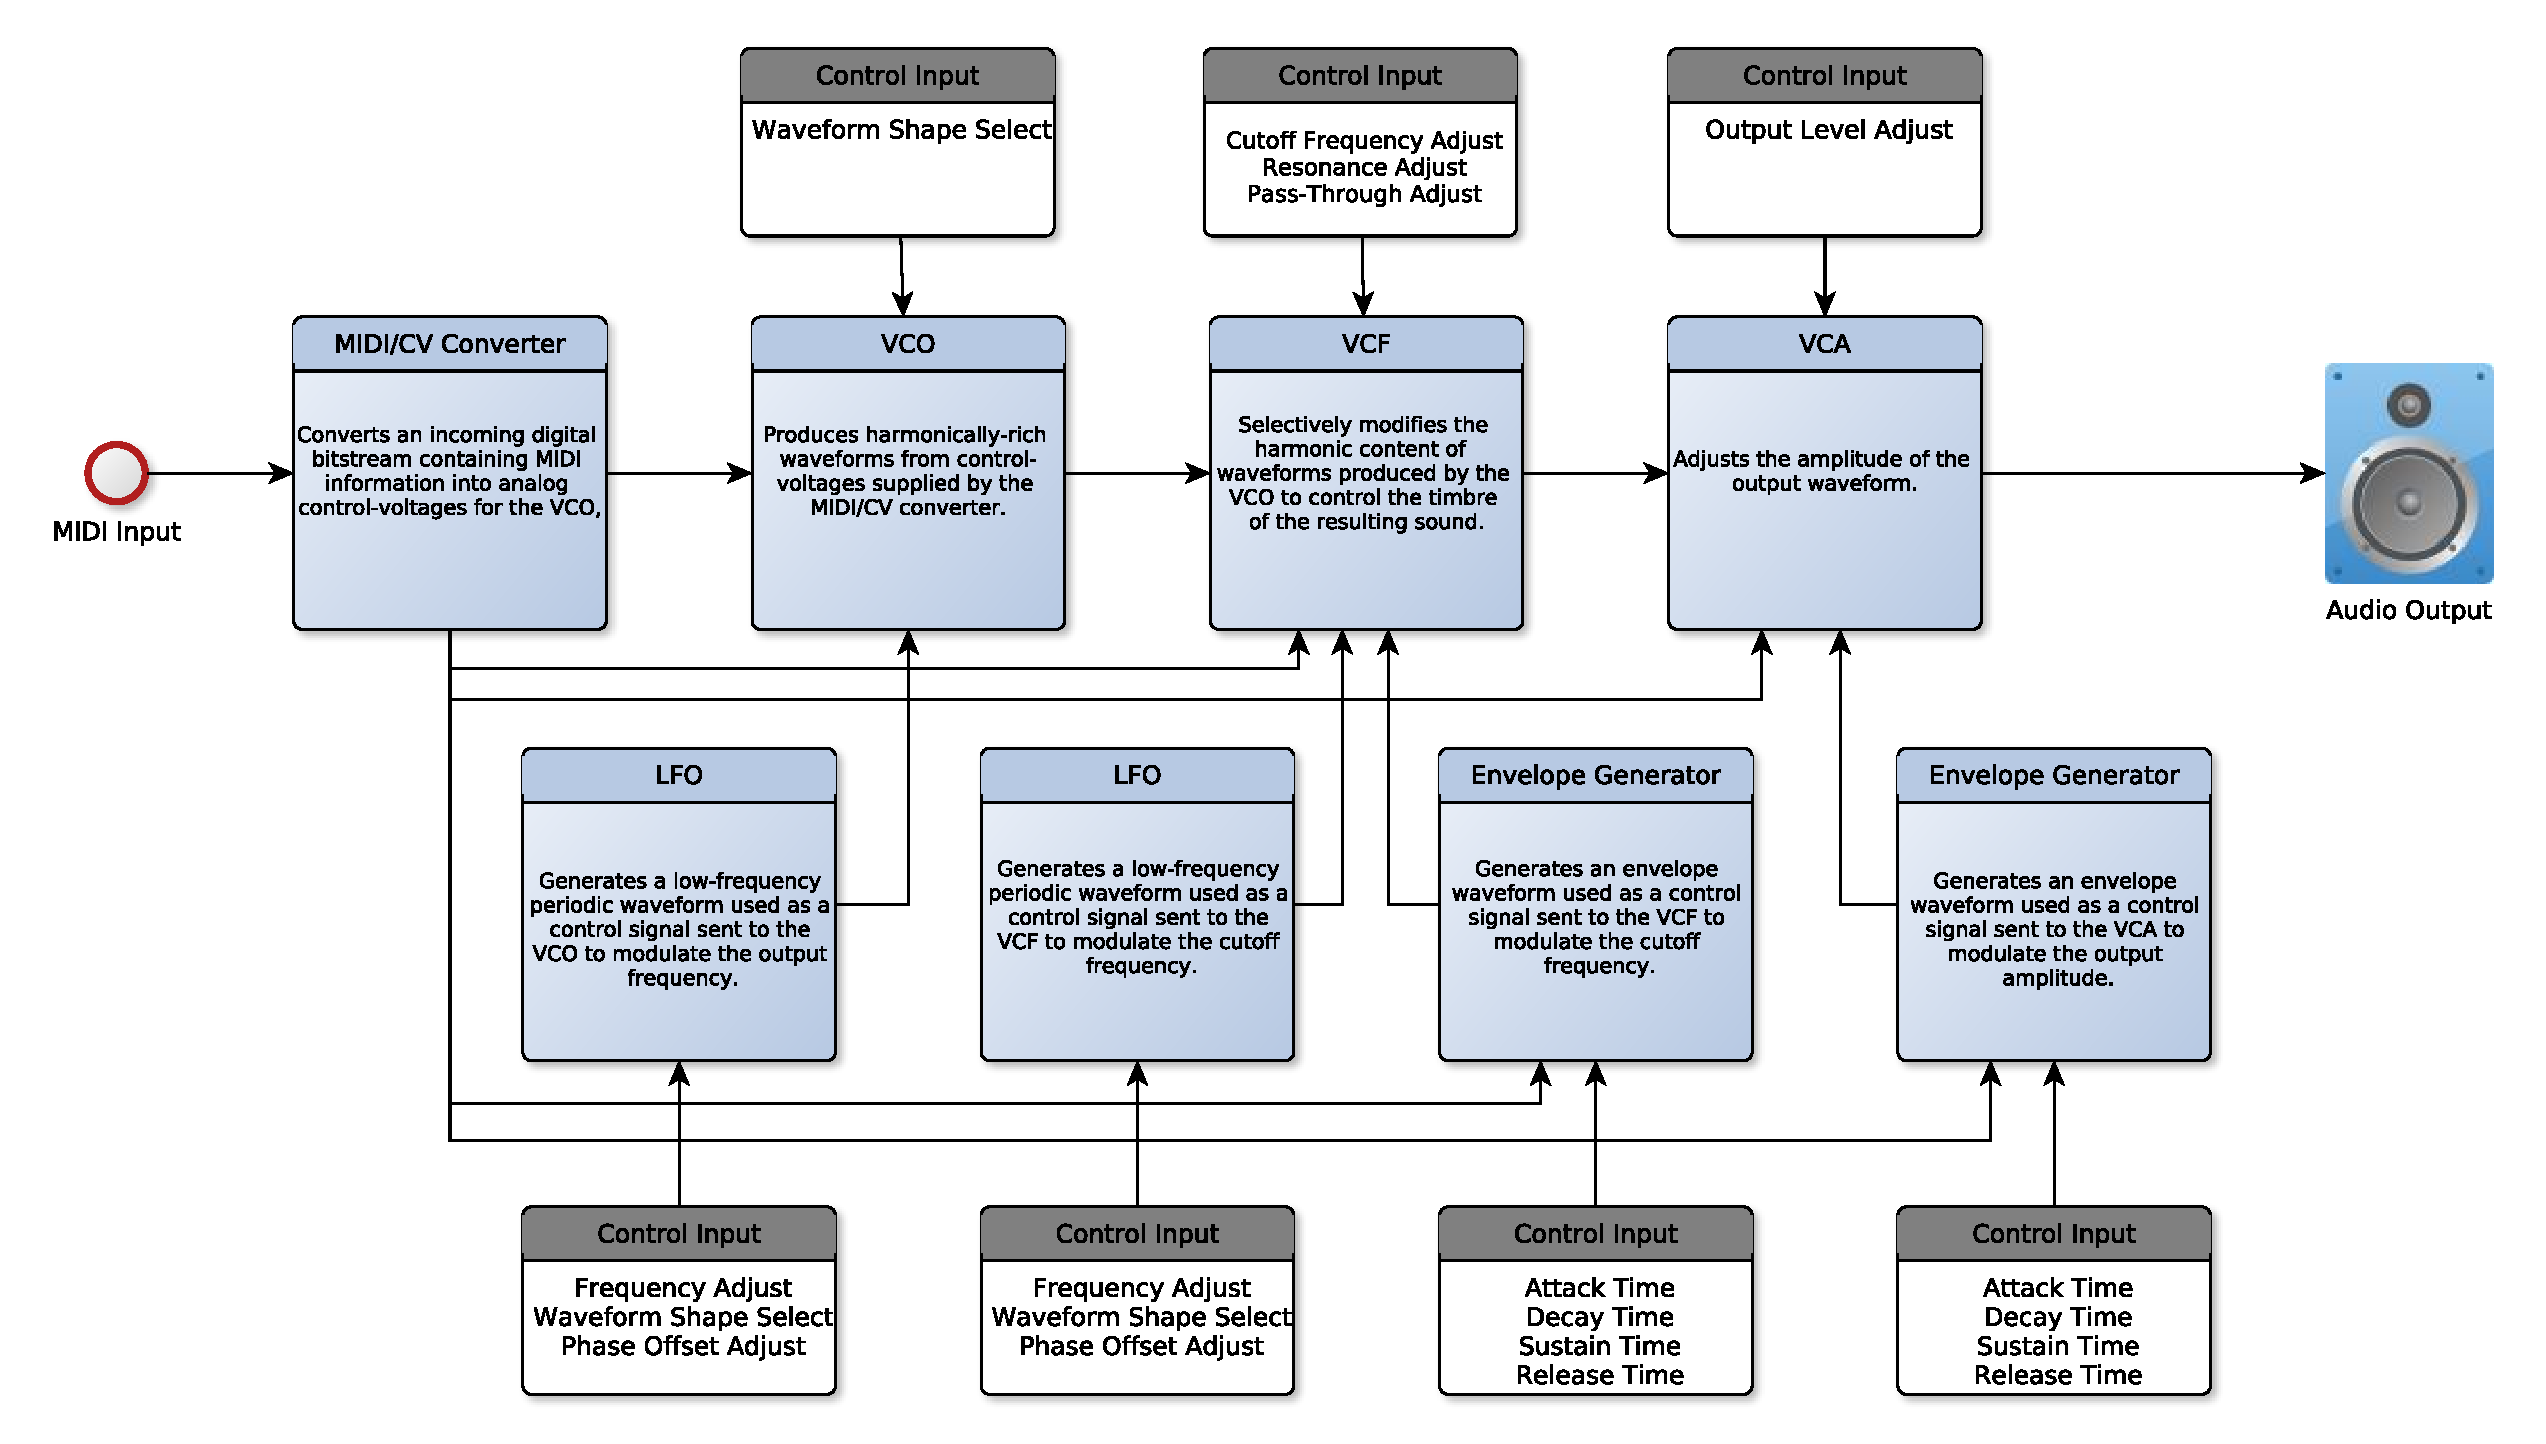
\includegraphics[width=\textwidth]{./figures/synthesizer.eps}
					\caption{Selectable Pitch Glide}
					\label{fig:selectable_pitch_glide}
				\end{figure}

			\subsubsection{Non-Inverting Amplifier}
				The last section in the output stage is a non-inverting amplifier, with a gain $A=2.2$. The amplifier scales the DAC output signal level from $0-5V$ to the $1V/$oct levels expected by the synthesizer VCO section. Texas Instruments' TL072 (Dual Low-Noise JFET-Input General-Purpose Operational Amplifier) was chosen for its high availability and low cost. Since rail-to-rail input/output operation is not required in this design, the 4V headroom between the +15V supply rail and the required maximum output voltage of $11V$ is more than sufficient to accommodate the ~$1.5V$ difference between the maximum supply voltage and maximum output voltage for the TL072. The non-inverting amplifier section is in standard configuration, with gain calculated by:
				\begin{equation}
					A = \frac{V_{out}}{V_{in}} = 1 + \frac{R8}{R7}
				\end{equation}
				\begin{figure}[H]
					%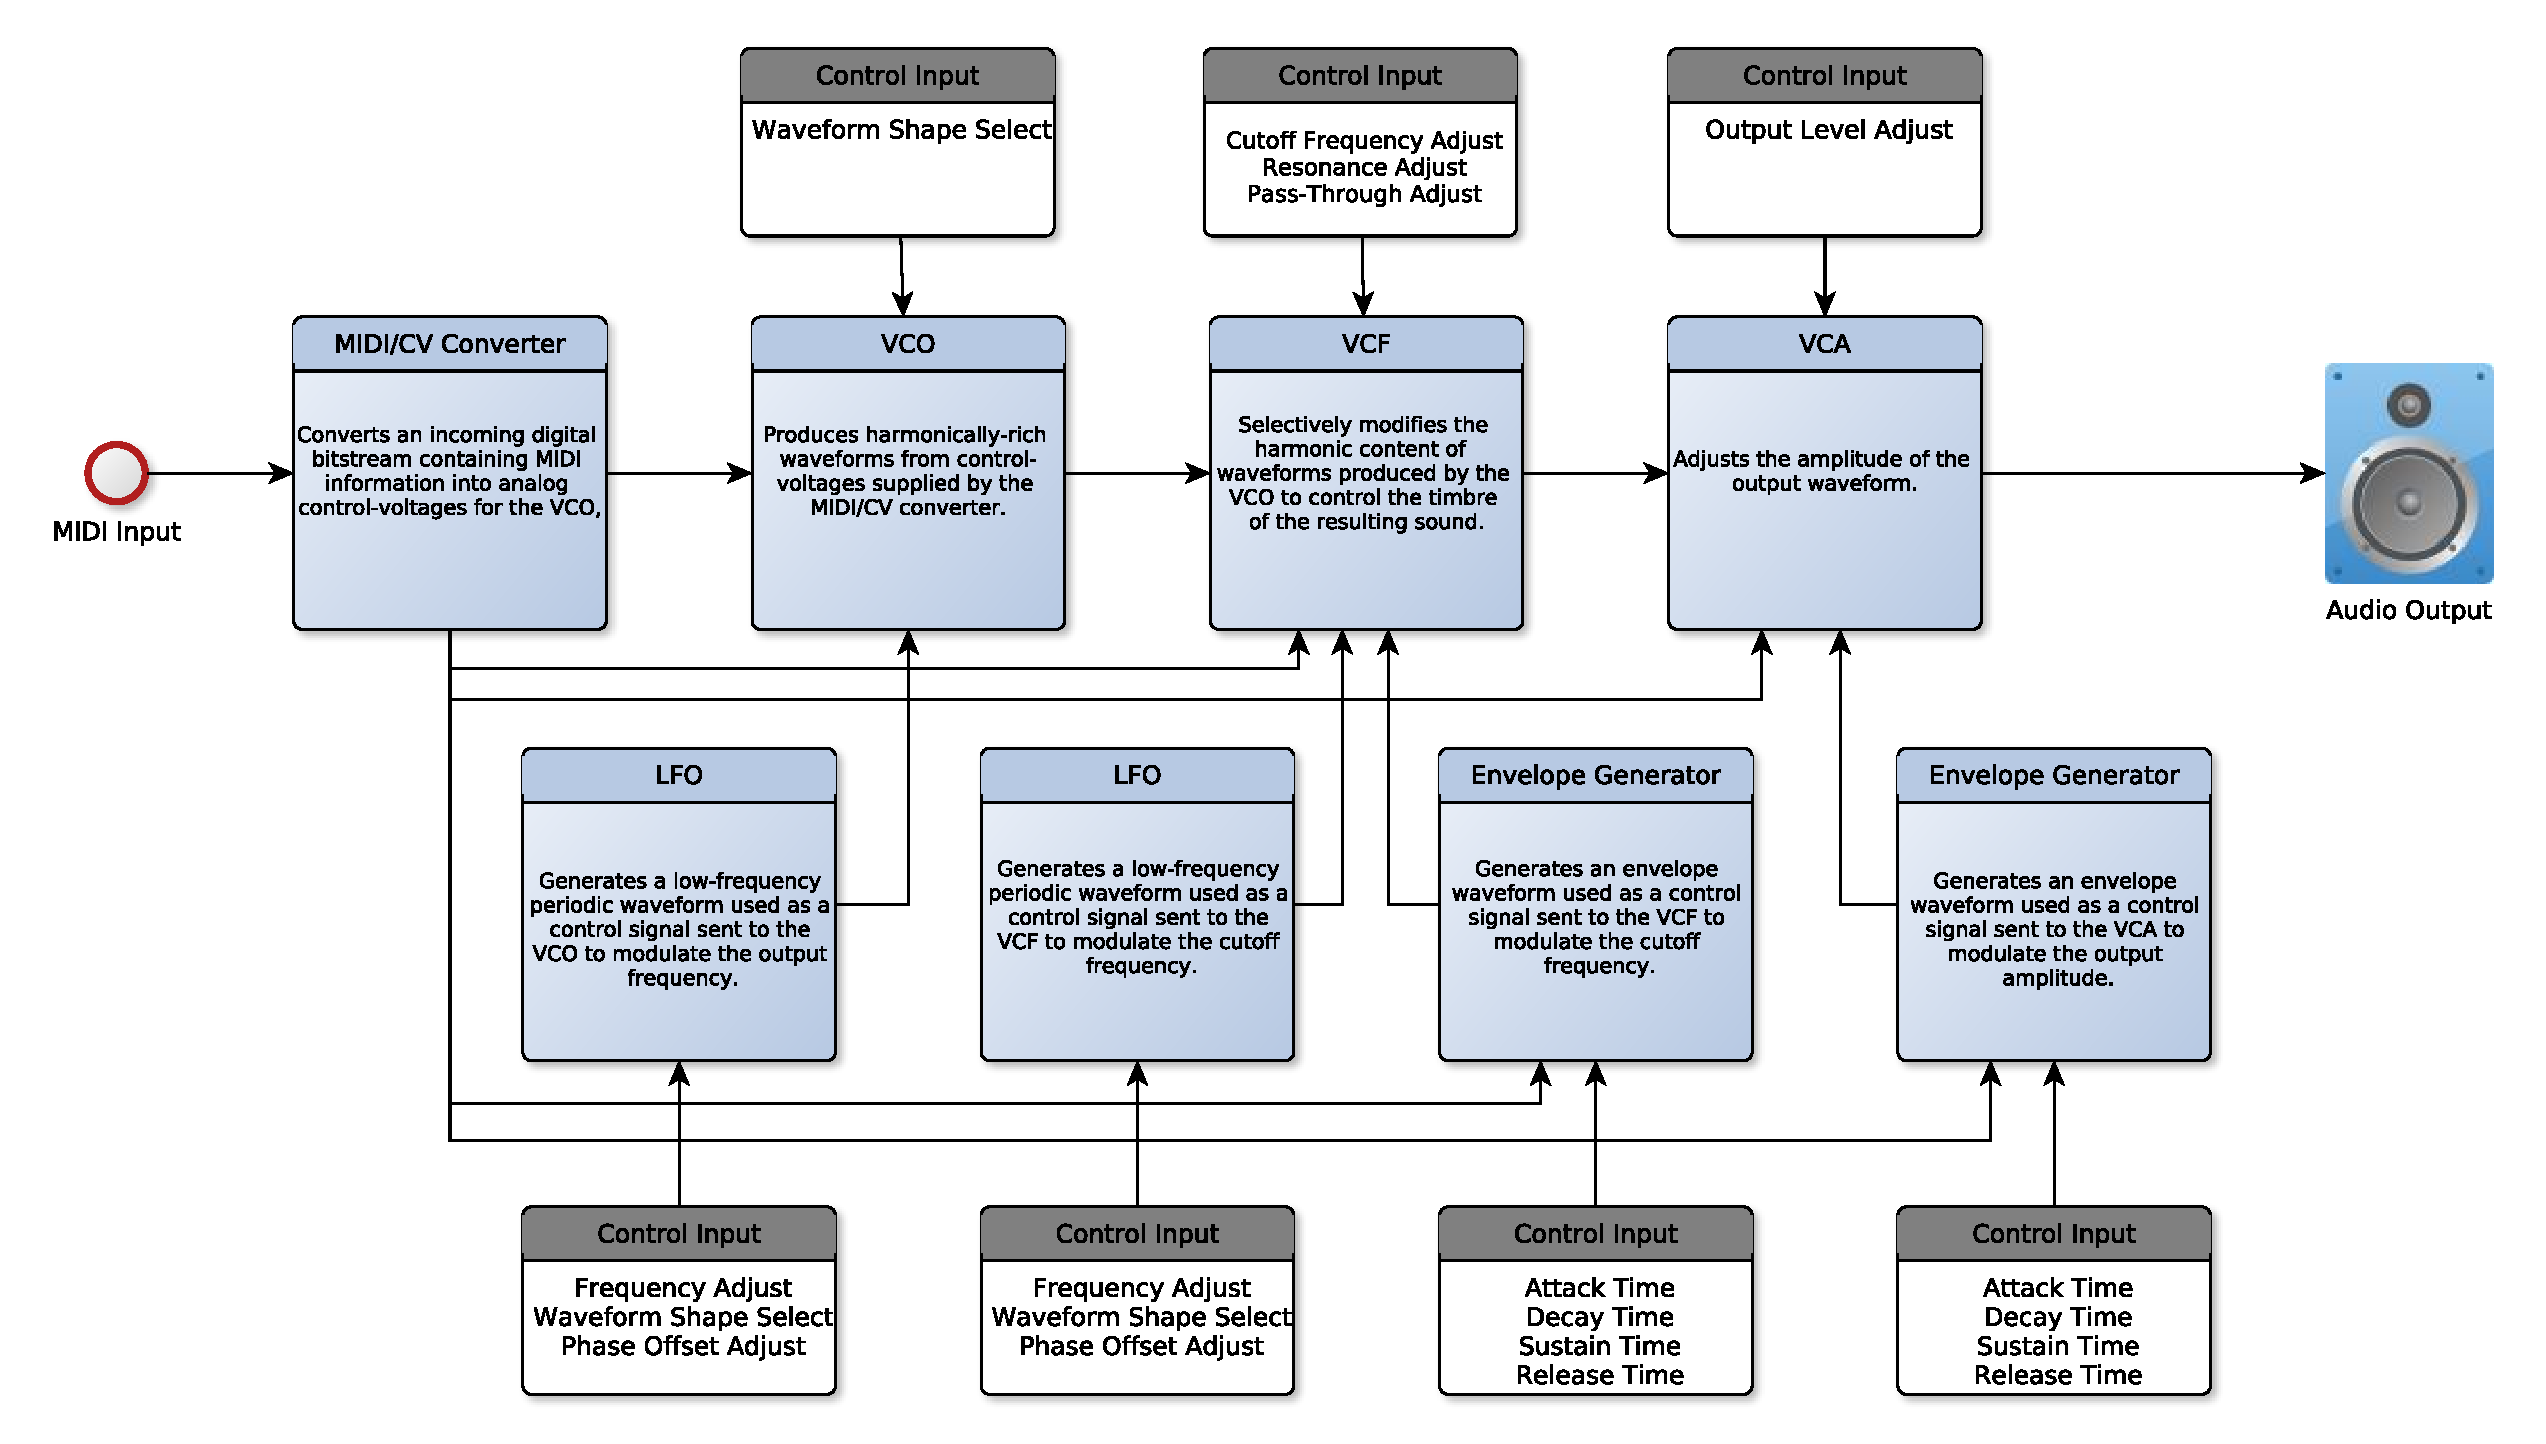
\includegraphics[width=\textwidth]{./figures/synthesizer.eps}
					\caption{Non-Inverting Amplifier}
					\label{fig:non-inverting_amplifier}
				\end{figure}

	\section{Software}
		The intent of this research is to learn more about the practical applications of the basic analog circuits discussed in this course, and to gain insight into the unique ways in which those basic analog circuits are applied in combination for the purpose of sound generation. It is also hoped that the basic circuit designs created during the completion of this project will provide the foundations for future revisions of this synthesizer, each of which will extend the range of achievable sounds, and allow for greater musical expression. 
\end{document}